\section{Turning}
	\subsection{Setup}
		\begin{figure}[ht!]
	\caption{Diagram of what happens when Alice turns.}
	\label{fig:turningAlice}
	\centering
	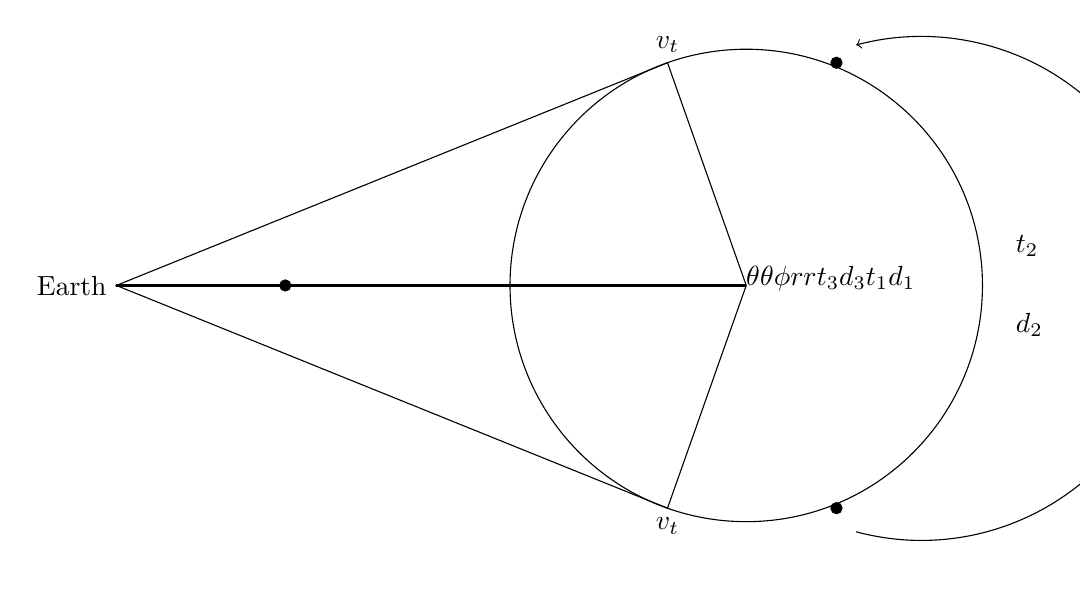
\begin{tikzpicture}
		\coordinate (O) at (0,0);
		\coordinate [label=left:Earth] (E) at (-8,0);
		\coordinate [label=above:$v_t$] (A) at (-1,2.828427125);
		\coordinate [label=below:$v_t$] (B) at (-1,-2.828427125);
		\coordinate [label=right:$\Del t_2$] (T) at (3.3,0.5);
		\coordinate [label=right:$\Del d_2$](D) at (3.3,-0.5);

		\draw (O) circle (3);
		\draw (A) -- (O) -- (B) -- (E) -- cycle;
		\draw[thick](O) -- (E);

		\tkzMarkRightAngle(E,A,O);
		\tkzMarkRightAngle(E,B,O);

		\tkzMarkAngle[size=0.6](A,O,E);
		\tkzLabelAngle(A,O,E){$\theta$};

		\tkzMarkAngle[size=0.6](E,O,B);
		\tkzLabelAngle[pos=-1](E,O,B){$\theta$};

		\tkzMarkAngle[size=0.75](B,O,A);
		\tkzLabelAngle(B,O,A){$\phi$};

		\tkzLabelSegment[above right](O,A){$r$};
		\tkzLabelSegment[below right](O,B){$r$};

		\tkzLabelSegment[above=1.25em](E,A){$\Del t_3$};
		\tkzLabelSegment[above=0.25em](E,A){$\Del d_3$};

		\tkzLabelSegment[below=0.25em](E,B){$\Del t_1$};
		\tkzLabelSegment[below=1.25em](E,B){$\Del d_1$};

		\draw[->] (-0.75,-3.128427125) arc (-105:105:3.2);

		\filldraw[black] (A) circle (2pt);
		\filldraw[black] (B) circle (2pt);
		\filldraw[black] (E) circle (2pt);
	\end{tikzpicture}
\end{figure}

		\[\Del t_1 = \Del t_3\]
		\[\Del d_1 = \Del d_3\]
		\subsubsection{Known values}
			\begin{description}
				\item[$a$] The acceleration.
				\item[\si{\clight}] The speed of light.
				\item[$T_T$] The total time.
			\end{description}
	\subsection{Calculations}
		\begin{samepagecols}{2}
			\subsubsection{Acceleration distance}
			\begin{align*}
				v &= \si{\clight}\tanh\left(\frac{at}{\si{\clight}}\right)\\
				v_t &= \si{\clight}\tanh\left(\frac{a \Del t_1}{\si{\clight}}\right)\\
				\Del d_1 &= \int \si{\clight}\tanh\left(\frac{a \Del t_1}{\si{\clight}}\right) \dif \Del t_1\\
				\Del d_1 &= \int \frac{\si{\clight}}{a} \times \frac{\sinh\left(\frac{a \Del t_1}{\si{\clight}}\right)}{\cosh\left(\frac{a \Del t_1}{\si{\clight}}\right)} \dif \Del t_1\\
				\Del d_1 &= \frac{\si{\clight}^2}{a} \int \frac{1}{\frac{\sinh\left(\frac{a \Del t_1}{\si{\clight}}\right)}{\cosh\left(\frac{a \Del t_1}{\si{\clight}}\right)}} \dif \Del t_1\\
				\Del d_1 &= \frac{\si{\clight}^2}{a} \ln\left| \cosh\left(\frac{1 \Del t_1}{\si{\clight}}\right)\right|\\
				&\frac{a \Del t_1}{\si{\clight}} > 0 \implies \cosh > 0\\
				\Del d_1 &= \frac{\si{\clight}^2}{a} \ln\left(\cosh\left(\frac{1 \Del t_1}{\si{\clight}}\right)\right)
			\end{align*}
			\columnbreak
			\subsubsection{Turn distance}
				\begin{align*}
					\tan \theta &= \frac{\Del d_1}{r}\\
					\theta &= \arctan\left(\frac{\Del d_1}{r}\right)
				\end{align*}
				\begin{equation*}
					\phi = 2\pi - 2\theta
				\end{equation*}
				\begin{equation*}
					\Del d_2 = \phi r
				\end{equation*}
			\subsubsection{Turn time}
				\begin{equation*}
					\Del t_2 = \frac{\Del d_2}{v_t}
				\end{equation*}
			\subsubsection{Turn radius}
				\begin{equation*}
					a = \frac{v^2}{r} \qquad r = \frac{v^2}{a}
				\end{equation*}
		\end{samepagecols}
	\newpage
	\subsection{The total time}
		\[\Del t_1 = \Del t_3\]
		\begin{align*}
			\Del T_T &= \Del t_1 + \Del t_2 + \Del t_s\\
			\Del T_T &= 2\Del t_1 + \Del t_2\\
			\Del T_T &= 2\Del t_1 + \frac{\left(2\pi - 2\arctan\left(\frac{\Del d_1}{r}\right)\right) \frac{v^2}{a}}{v}\\
			\Del T_T &= 2\Del t_1+\frac{\left(2\pi - 2\arctan\left(\frac{\frac{\si{\clight}^2}{a}\ln\left(\cosh\left(\frac{a\Del t_1}{\si{\clight}}\right)\right)}{\frac{v^2}{a}}\right)\right) v}{a}\\
			\Del T_T &= 2\Del t_1+\frac{\left(2\pi-2\arctan\left(\frac{\si{\clight}^2\ln\left(\cosh\left(\frac{a\Del t_1}{\si{\clight}}\right)\right)}{\left(\si{\clight}\tanh\left(\frac{a\Del t_1}{\si{\clight}}\right)\right)^2}\right)\right) \times \si{\clight}\tanh\left(\frac{a\Del t_1}{\si{\clight}}\right)}{a}
		\end{align*}
		Trying to solve for $\Del t_1$ will lead us to a world of pain, so instead we will use a computer to solve it.

		The program to solve it was written by David White, and the source code is in appendix \vref{appendix:sourceCode}.
